\documentclass[UTF8]{book}
\usepackage{ctex}
\usepackage{amsmath}
\usepackage{bm}
\usepackage{makeidx}
\usepackage{enumitem}
\usepackage{rotating} 
\usepackage{yhmath}
\usepackage{textcomp,booktabs}
\usepackage[usenames,dvipsnames]{color}
\usepackage{colortbl}
\usepackage{makecell}
\usepackage{gensymb}
\usepackage{cancel}
\usepackage{graphicx}
\usepackage{pifont}
\usepackage[all,pdf]{xy}
\usepackage{exscale}
\usepackage{blindtext}
\usepackage{hyperref}
\hypersetup{
colorlinks=true,
linkcolor=black
}
\usepackage{nameref}
\usepackage{relsize}
\usepackage{titlesec}
\usepackage{ifthen}
\usepackage{array}
\usepackage[flushleft]{threeparttable}
\usepackage{diagbox}
\usepackage{mathtools}
\usepackage{amsfonts}
\usepackage{bbm}
\usepackage{ulem}
\usepackage{xcolor}
\usepackage{color}
\usepackage{mathptmx}
\usepackage{amssymb}
\usepackage{geometry}
\geometry{a4paper, left=2.54cm,right=2.54cm,top=2.54cm,bottom=2.54cm}
%\geometry{b5paper, left=1.6cm,right=2cm,top=2cm,bottom=2cm}
\usepackage{mathrsfs}
\usepackage{tikz,tkz-euclide}
\usepackage{tikz}
\usetikzlibrary{patterns}
\usetikzlibrary{shapes,arrows}
\usepackage{esvect}
\usepackage{fancyhdr}
\pagestyle{fancy}
\fancyhead{} % clear all fields 
\cfoot{}
\fancyhead[LE,RO]{\thepage} 
\renewcommand{\headrulewidth}{0pt}
\renewcommand{\footrulewidth}{0pt}
\linespread{1.4}
\date{}
\graphicspath{ {Graphs} }
\usepackage{listings}
\usepackage{color}

\definecolor{dkgreen}{rgb}{0,0.6,0}
\definecolor{gray}{rgb}{0.5,0.5,0.5}
\definecolor{mauve}{rgb}{0.58,0,0.82}

\lstset{
  basicstyle=\ttfamily,
  columns=fullflexible,
  frame=single,
  breaklines=true,
  backgroundcolor=\color{gray!20!white}
}
\definecolor{codegray}{gray}{0.8}
\newcommand{\code}[1]{\colorbox{codegray}{\texttt{#1}}}
%通用:
\newcounter{mylabelcounter}
\makeatletter
\newcommand{\labeltext}[2]{%
#1\refstepcounter{mylabelcounter}%
\immediate\write\@auxout{%
  \string\newlabel{#2}{{1}{\thepage}{{\unexpanded{#1}}}{mylabelcounter.\number\value{mylabelcounter}}{}}%
}%
}
%Xsum
\DeclareFontFamily{U} {cmex}{}
\DeclareFontShape{U}{cmex}{m}{n}{
  <-6> cmex5
  <6-7> cmex6
  <7-8> cmex7
  <8-9> cmex8
  <9-10> cmex9
  <10-12> cmex10
  <12-> cmex12}{}
\DeclareSymbolFont{Xcmex} {U} {cmex}{m}{n}
\DeclareMathSymbol{\Xdsum}{\mathop}{Xcmex}{88}
\DeclareMathSymbol{\Xtsum}{\mathop}{Xcmex}{80}
\DeclareMathOperator*{\Xsum}{\mathchoice{\Xdsum}{\Xtsum}{\Xtsum}{\Xtsum}}
%Xsum
%choice
\newcommand{\fourch}[4]{%~\hfill(\qquad)\\
\begin{tabular}{*{4}{@{}p{0.25\textwidth}}}(A)~#1 & (B)~#2 & (C)~#3 & (D)~#4\end{tabular}}
\newcommand{\twoch}[4]{%~\hfill(\qquad)\\
\begin{tabular}{*{2}{@{}p{0.5\textwidth}}}(A)~#1 & (B)~#2\end{tabular}\\\begin{tabular}{*{2}{@{}p{0.5\textwidth}}}(C)~#3 & (D)~#4\end{tabular}}
\newcommand{\onech}[4]{%~\hfill(\qquad)\\
(A)~#1 \\ (B)~#2 \\ (C)~#3 \\ (D)~#4}
 
\newlength\widthcha
\newlength\widthchb
\newlength\widthchc
\newlength\widthchd
\newlength\widthch
\newlength\tabmaxwidth
\setlength\tabmaxwidth{1\textwidth}
\newlength\fourthtabwidth
\setlength\fourthtabwidth{0.25\textwidth}
\newlength\halftabwidth
\setlength\halftabwidth{0.5\textwidth}
\newcommand{\choice}[4]{\settowidth\widthcha{AM.#1}\setlength{\widthch}{\widthcha}
    \settowidth\widthchb{BM.#2}
    \ifthenelse{\widthch<\widthchb}{\setlength{\widthch}{\widthchb}}{}
    \settowidth\widthchb{CM.#3}
    \ifthenelse{\widthch<\widthchb}{\setlength{\widthch}{\widthchb}}{}
    \settowidth\widthchb{DM.#4}
    \ifthenelse{\widthch<\widthchb}{\setlength{\widthch}{\widthchb}}{}
    \ifthenelse{\widthch<\fourthtabwidth}{\fourch{#1}{#2}{#3}{#4}}
    {\ifthenelse{\widthch<\halftabwidth\and\widthch>\fourthtabwidth}{\twoch{#1}{#2}{#3}{#4}}
        {\onech{#1}{#2}{#3}{#4}}}}
%choice
% Default fixed font does not support bold face
\DeclareFixedFont{\ttb}{T1}{txtt}{bx}{n}{12} % for bold
\DeclareFixedFont{\ttm}{T1}{txtt}{m}{n}{12}  % for normal

% Custom colors
\usepackage{color}
\definecolor{deepblue}{rgb}{0,0,0.5}
\definecolor{deepred}{rgb}{0.6,0,0}
\definecolor{deepgreen}{rgb}{0,0.5,0}

\usepackage{listings}

% Python style for highlighting
\newcommand\pythonstyle{\lstset{
language=Python,
basicstyle=\ttm,
morekeywords={self},              % Add keywords here
keywordstyle=\ttb\color{deepblue},
emph={MyClass,__init__},          % Custom highlighting
emphstyle=\ttb\color{deepred},    % Custom highlighting style
stringstyle=\color{deepgreen},
frame=single,                         % Any extra options here
showstringspaces=false
}}


% Python environment
\lstnewenvironment{python}[1][]
{
\pythonstyle
\lstset{#1}
}
{}

% Python for external files
\newcommand\pythonexternal[2][]{{
\pythonstyle
\lstinputlisting[#1]{#2}}}

% Python for inline
\newcommand\pythoninline[1]{{\pythonstyle\lstinline!#1!}}
%%%%%
% Bash style for highlighting
\newcommand\bashstyle{\lstset{
language=bash,
basicstyle=\ttm\normalsize,
tabsize=4,
morekeywords={self, head, tail, uniq, sort, grep, cat, cut, echo, wc, cp, rm, mkdir, cd, nano, man, ls, history, bash, rmdir, find, plink, bcftools, bedtools, octopus},              % Add keywords here
keywordstyle=\color{deepblue}\normalsize\bfseries,
emph={MyClass,__init__},          % Custom highlighting
emphstyle=\ttb\color{deepred},    % Custom highlighting style
stringstyle=\color{deepgreen},
frame=single,                         % Any extra options here
showstringspaces=false
}}


% Python environment
\lstnewenvironment{bash}[1][]
{
\bashstyle
\lstset{#1}
}
{}

% Python for external files
\newcommand\bashexternal[2][]{{
\bashstyle
\lstinputlisting[#1]{#2}}}

% Python for inline
\newcommand\bashinline[1]{{\bashstyle\lstinline!#1!}}
%%%%%
\newcommand{\dollar}{\mbox{\textdollar}}
\newcommand{\dps}[1]{\ensuremath{\displaystyle{#1}}}
\newcommand\ffrac[2]{\ensuremath{\dfrac{\;#1\;}{\;#2\;}}}
\newcommand{\comma}{\, \; \;\mathclap{\text{,}}} %用于mathmode中的逗号
\newcommand{\semicolon}{\, \; \;\mathclap{\text{;}}} %用于mathmode中的分号
\newcommand{\pl}{\phantom{l}} %用来占位
\newcommand{\un}{\ding{172}}
\newcommand{\deux}{\ding{173}}
\newcommand{\trois}{\ding{174}}
\newcommand{\quatre}{\ding{175}}
\newcommand{\et}{&}
\newcommand{\f}{^2}
\newcommand{\xz}{(\qquad)}
\newcommand{\tk}{\underline{\qquad\qquad}}
%高等数学:
\renewcommand{\d}{\,\mathrm{d}}
\newcommand{\dt}{\,\mathrm{d}t}
\newcommand{\dr}{\,\mathrm{d}r}
\newcommand{\du}{\,\mathrm{d}u}
\newcommand{\dv}{\,\mathrm{d}v}
\newcommand{\dx}{\,\mathrm{d}x}
\newcommand{\dy}{\,\mathrm{d}y}
\newcommand{\dz}{\,\mathrm{d}z}
\newcommand{\df}{\,\mathrm{d}f}
\newcommand{\bigmid}{\, \bigg | \,} %用于集合中有分数的情况
\newcommand\matharr{\tikz[baseline=-0.4ex]\draw[-stealth] (0,0) -- + (3mm,0);} %用于下标中的右箭头
\newcommand\textarr{\; \tikz[baseline=-0.55ex]\draw[-stealth] (0,0) -- + (4mm,0);} %用于文本中的右箭头,注意用占位符调整前后间距
\newcommand{\limite}[2]{\ensuremath{\lim\limits_{#1\matharr #2}}} %#1趋向于#2
\newcommand{\dlimite}[4]{\ensuremath{\displaystyle{\lim_{\substack{ \phantom{l}#1\matharr #2\phantom{l} \\ #3\matharr #4}}}}} %#重极限:1趋向于#2,#3趋向于#4,phantom{l}用来占位
\newcommand{\neighbr}{\ensuremath{\mathring{U}(x_0\comma \delta)}} %去心邻域U
\newcommand{\neighbor}{\ensuremath{U(x_0\comma \delta)}} %邻域U
\newcommand{\tikzrm}[1]{
	\fill[white] #1 circle(1.5pt);
	\draw #1 circle(1.5pt);
}
\newcommand{\derivee}[4]{
	\ffrac{\,\mathrm{d}^{#1}#2}{\,\mathrm{d}#3^{#4}}
}
\newcommand{\intscript}[2]{\biggl.\biggr|_{\, #2}^{\, #1}} %求出原函数以后代入的积分上下限
\newcommand{\concept}[1]{\textcolor{magenta}{#1}}
\renewcommand{\emph}[1]{\textcolor{blue}{#1}}
\newcommand{\dint}[2]{\ensuremath{\displaystyle{\int_{#2}^{#1}}}}
\newcommand{\diint}[4]{\ensuremath{\displaystyle{\int_{#2}^{#1}\int_{#4}^{#3}}}}
\newcommand{\bint}{\mathlarger{\int}} %用于将幂次上的积分号放大
\newcommand{\exiint}{\ensuremath{\!\!\!}} %用于缩短累次积分中积分号的距离
\newcommand{\fxy}{\ensuremath{f(x\comma y)}}
\newcommand{\xoyo}{\ensuremath{(x_0\comma y_0)}}
\newcommand{\series}{\ensuremath{\dps{\Xsum_{n=1}^\infty}}} %级数
\newcommand{\serieso}{\ensuremath{\dps{\Xsum_{n=0}^\infty}}} %0开始的级数
%线性代数:
\newcommand{\pA}{\ensuremath{\pmb{A}}}
\newcommand{\pB}{\ensuremath{\pmb{B}}}
\newcommand{\pC}{\ensuremath{\pmb{C}}}
\newcommand{\pO}{\ensuremath{\pmb{O}}}
\newcommand{\pP}{\ensuremath{\pmb{P}}}
\newcommand{\pQ}{\ensuremath{\pmb{Q}}}
\newcommand{\pE}{\ensuremath{\pmb{E}}}
\newcommand{\px}{\ensuremath{\pmb{x}}}
\newcommand{\pX}{\ensuremath{\pmb{X}}}
\newcommand{\pR}{\ensuremath{\pmb{R}}}
\newcommand{\pZ}{\ensuremath{\pmb{Z}}}
\newcommand{\pal}{\ensuremath{\pmb{\alpha}}}
\newcommand{\pbe}{\ensuremath{\pmb{\beta}}}
\newcommand{\pxi}{\ensuremath{\pmb{\xi}}}
\newcommand{\pet}{\ensuremath{\pmb{\eta}}}
\renewcommand{\t}{\ensuremath{^\mathrm{T}}}
\newcommand\laarr{\qquad\tikz\draw[-stealth] (0,0) -- + (7mm,0);\qquad} %用于矩阵中的初等变换
\newcommand{\laarrt}[1]{\qquad\tikz\draw[-stealth] (0,0) -- (4mm,0) node[above]{#1}--+ (4mm,0);\qquad} %初等变换上带字
%概率:
\newcommand{\XY}{\ensuremath{(X\comma Y)}}
\newcommand{\Cov}{\ensuremath{\mathrm{Cov}}}
\newcommand{\cip}{\tikz[baseline=-0.55ex]\draw[-stealth] (0,0) -- (2mm,0) node[above]{$\;\;P$}--+ (4mm,0);\;} %依概率收敛
\newcommand{\seriesn}{\ensuremath{\dps{\Xsum_{i=1}^n}}} %1开始到n的连续求和
\begin{document}
\kaishu
\begin{center}
\Large{Fundamentals of Immunology Notes}
\end{center}
1.3\quad \textbf{Pathogen Varieties}
\begin{itemize}
\item Different types of pathogens:
\begin{itemize}
	\item Virus: Unstructured DNA, Protein Coating.
	\item Bacteria.
	\item Fungus.
	\item Unicellular Eukaryotes.
	\item Multicellular Worm.
\end{itemize}
\end{itemize}
1.4\quad \textbf{Pathogen Recognition}
\begin{itemize}
\item  Neutrophils attach to bacteria prior to phagocytizing them.
\item \concept{Lysozyme}, an enzyme that cuts up bacterial cell wall peptidoglycan.
\item Pore in pathogenic membrane constructed by complement MAC.
\item Leucine-rich hook domain found in many pattern recognition receptors.
\item Properties of Innate vs Adaptive Defenses:
\begin{center}
\begin{tabular}{|m{1.5cm}<{\centering}|m{3cm}<{\centering}|m{2cm}<{\centering}|m{3cm}<{\centering}|m{2cm}<{\centering}|} \Xhline{1.2pt}
Innate \et Fast:Minutes after exposure \et Always there \et Recognizes patterns: types of molecules that a pathogen might have and you would not have \et Neutrophils, macrophages, NK cells, proteins, barriers \\ \hline
Adaptive \et Slower: approximately two weeks after first exposure and three days after subsequent exposure \et requires gene rearrangement \et recognizes specific parts of proteins characteristic of a pathogen \et B cells, antibodies, T$_\mathrm{C}$ cells, T$_\mathrm{H}$ cells.\\ \Xhline{1.2pt}
\end{tabular}
\end{center}
\end{itemize}
1.7\quad Innate vs Defensive Responses
\begin{itemize}
\item Responding to foreign antigen:
\begin{center}
\begin{tabular}{|m{5.5cm}<{\centering}|m{4cm}<{\centering}|m{4cm}<{\centering}|} \Xhline{1.2pt}
Responding Cell \et $\mathrm{T_H}$ (Helper) \et $\mathrm{T_C}$ (Cytotoxic) \\ \hline
Response \et Coordinates immune response \et Attacks and kills cell\\ \hline
Binds antigen with \et $\alpha\beta$ T-cell receptor \et $\alpha\beta$ T-cell receptor\\ \hline
Co-receptor \et CD4 \et CD8\\ \hline
Antigen presented/displayed on \et Class II MHC \et Class I MHC\\ \hline
Cells presenting/displaying \et Sentinel dendritic, macrophages, B cells\et All nucleated cells except sperm\\ \hline
Source of antige \et phagocytosis \et synthesized in cell\\ \hline
Antigen hydrolyzed in \et phagolysosome \et proteosome\\ \Xhline{1.2pt}
\end{tabular}
\end{center}
\end{itemize}
2.1\quad Terminology
\begin{itemize}
\item The \concept{primary organs} are where the genes rearrange to make various recognition molecules. They include:
\begin{itemize}
	\item Bone marrow for B cells.
	\item Myeloid cell.
	\item Thymus for T cells. 
\end{itemize}
\item The \concept{secondary organs} are where the immune cells are activated and counter-antigen. They include:
\begin{itemize}
	\item Lymph nodes.
	\item Spleen.
	\item Regions of the gut.
\end{itemize}
\item Myeloid and lymphoid cells:
\begin{itemize}
	\item \concept{Myeloid cells} are all innate and are found everywhere.
	\item \concept{Lymphoid cells} are only present in lymphs, including B cells, T cells, NK cells, and sentinel dendritic cells.
\end{itemize}
\item \concept{Cluster of Differentiation (CD)} refers to how cells come out of various separation procedures that involve cytometry. Hence, CDx cells are only informative in the chronological order they were discovered.
\end{itemize}
2.2\quad Hematopoiesis
\begin{itemize}
\item \concept{Pluripotent stem cell} has many possible developmental phase.
\item Different blood cells:
\begin{itemize}
	\item \concept{Erythrocytes} or red blood cells:
	\begin{itemize}
		\item Makes up the majority of the cells.
		\item Minor cooperation with the immune system.
		\item Maintain oxygen supply and pH in blood.
	\end{itemize}
	\item \concept{Thrombocytes} or platelets:
	\begin{itemize}
		\item Little fragments cells.
		\item Pinched off from megakaryocytes.
		\item Help stimulate the immune system but not considered part of the white blood cells.
	\end{itemize}
	 \item \concept{Megakaryocytes}:
	 \begin{itemize}
	 	\item Produce platelets to repair blood vessels.
	 	\item Has thrombopoietin receptors, whose activation urges the up-regulation of platelets.
	 \end{itemize}
\end{itemize}
\item Workflow of a hematopoietic stem cell:
\begin{center}
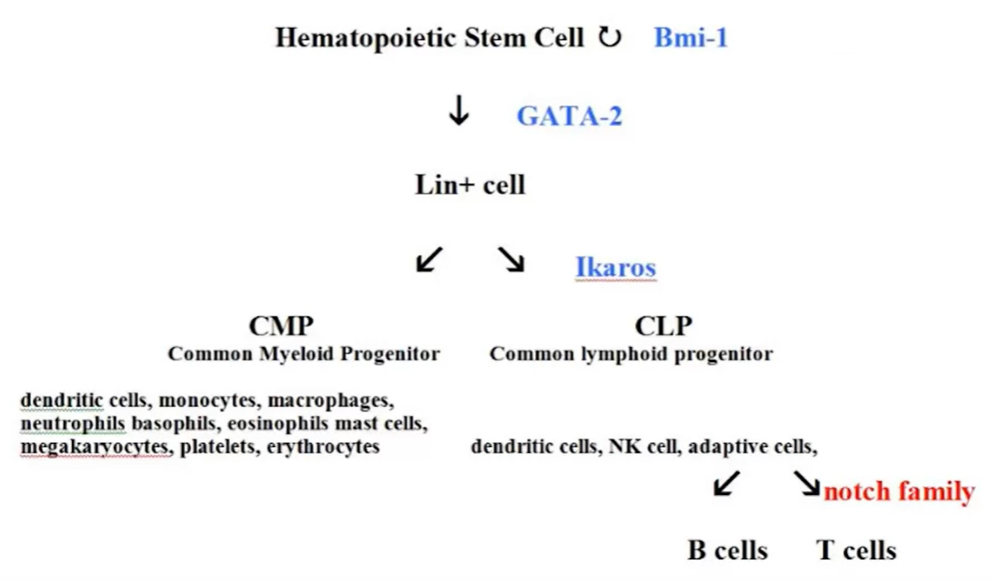
\includegraphics[scale=0.5]{2.2.1.png}
\end{center}
\end{itemize}
\end{document}
